\documentclass[twocolumn]{aastex6}

\usepackage{marginnote}

% alternate micron command
\newcommand{\um}{\micron}

% referencing commands
\newcommand{\sref}[1]{Sec.~\ref{#1}}

% commands and packages that shouldn't be needed in final version
\usepackage{xcolor, soul}
\newcommand{\todo}[1]{\textcolor{red}{TODO: #1}}
\newcommand{\note}[1]{\textcolor{red}{Note: #1}}
\newcommand{\ascl}[1]{\href{http://www.ascl.net/#1}{ascl:#1}}
\newcommand{\status}[1]{\textsf{#1}}

\usepackage{hyperref}
\hypersetup{pdftex,colorlinks=true,allcolors=blue, bookmarks=true}


\shorttitle{JCMT LR1: SCUBA-2 850\micron}
\shortauthors{SF Graves et al.}


\begin{document}
\title{The JCMT Legacy Release 1: SCUBA-2 850\micron\ observations}

\author{Sarah F. Graves\altaffilmark{1,2},
     Graham S. Bell\altaffilmark{1},
     David S. Berry\altaffilmark{1},
     Iain M. Coulson\altaffilmark{1},
     Malcolm Currie\altaffilmark{1,3},
     Jessica T. Dempsey\altaffilmark{1},
     Per Friberg\altaffilmark{1},
     Tim Jenness\altaffilmark{3},
     Doug Johnstone\altaffilmark{3},
     Harriet A. L. Parsons\altaffilmark{1},
     Mark G. Rawlings\altaffilmark{1},
     Holly S. Thomas\altaffilmark{4},
    and Jan G. A. Wouterloot\altaffilmark{1}
}
\altaffiltext{1}{East Asian Observatory, 660 N.\ A`oh\=ok\=u Place,Hilo, HI 96720, USA}
\altaffiltext{2}{s.graves@eaobservatory.org}
\altaffiltext{3}{Insert other affiliations}
\altaffiltext{4}{Joint Astronomy Centre, 660 N.\ A`oh\=ok\=u Place,Hilo, HI 96720, USA}

\begin{abstract}
  % Re write this properly once the rest of the paper is written.
  The JCMT Science Archive allows access to raw and reduced data for
  all publicly available JCMT observations. To aid users of JCMT
  products, we have produced a standardised reduction of public JCMT
  SCUBA-2 850\,\um\ observations. These reductions provide
  uniformly reduced co-additions of of all standard, public data
  observed before 2015 March 1st, as well as catalogues to identify
  the regions where emission was detected. The data have been gridded
  in the HEALPix HPX scheme.
\end{abstract}

\keywords{submillimeter:general; catalogs}

\section{Introduction}
\todo{Shorten this section?}

% JCMT & SCUBA-2
The JCMT is a 15\,m submillimetre telescope located at an altitude of
4092\,m on Mauna Kea, where it has been operating since
1987. Its current instrument suite includes SCUBA-2, a 10,000
pixel continuum camera that observes simultaneously at 450\,\um\ and
850\,\um\ wavelengths \citep{Holland2013}.

% Whats in the Archive -- reductions using PI-chosen configurations
The JCMT Science Archive \citep{2015Economou}, hosted by the Canadian
Astronomy Data Centre (CADC) contains both raw, instrumental-format
data and pipeline-reduced FITS-format data. All science observations
from the observatory are reduced each night using the PI's chosen
configuration.  These reduced observations and co-adds are then
automatically made available in the archive (initially just to the PI
and coIs, but then publicly once the observations are no longer
proprietary). Although these project-specific configurations are vital
to ensure PI's can access the most scientifically useful reductions of
their data, it means that the reduced archival data is considerably
more heterogenous than some astronomical users may suspect, and
reduced observations of the same region of sky from different projects
cannot be naively co-added together. Despite this, \citet{Bell2014}
found that more than fifty percent of papers using JCMT data made use
of archive data.

To maximise the scientific return on the many years of archival data,
% and to make it as easy as possible for non-submm-experts to use the
% JCMT data,
the Joint Astronomy Centre, then-operators of the JCMT, decided to
produce `legacy' reductions of all public data from the current
instrumentation. This work has been continued.These legacy reductions
were envisioned as providing a uniform, standardised reduction,
co-addition and source detection of all publicly available
observations. The aim was to produce uniformly reduced high quality
co-added maps that required as little checking as possible by hand,
and would allow astronomers to easily discover which regions have been
observed, the noise levels in existing regions, and where there are
clear detections. This paper presents the first release in this
project: the 850\,\um\ SCUBA-2 continuum observations. Planned future
releases are the 450\,\um\ SCUBA-2 observations and HARP spectral
cubes.


% Release of block 1 and this data
This release includes data taken from 2011 February 2 to 2015 March
1st, when the JCMT was began to be operated by East Asian Observatory.
The first block of this data, from 2011 to Augst 1st 2013 was already
reduced and publicly released in September 2015. This release includes
these same reduced individual observations, reductions of the newer
data taken up until March 2015, and new coadds and catalogs produced
from all the data (and using a slightly different calibration
constant).




\subsection{Overview of Release}

\begin{figure*}
  \centering
  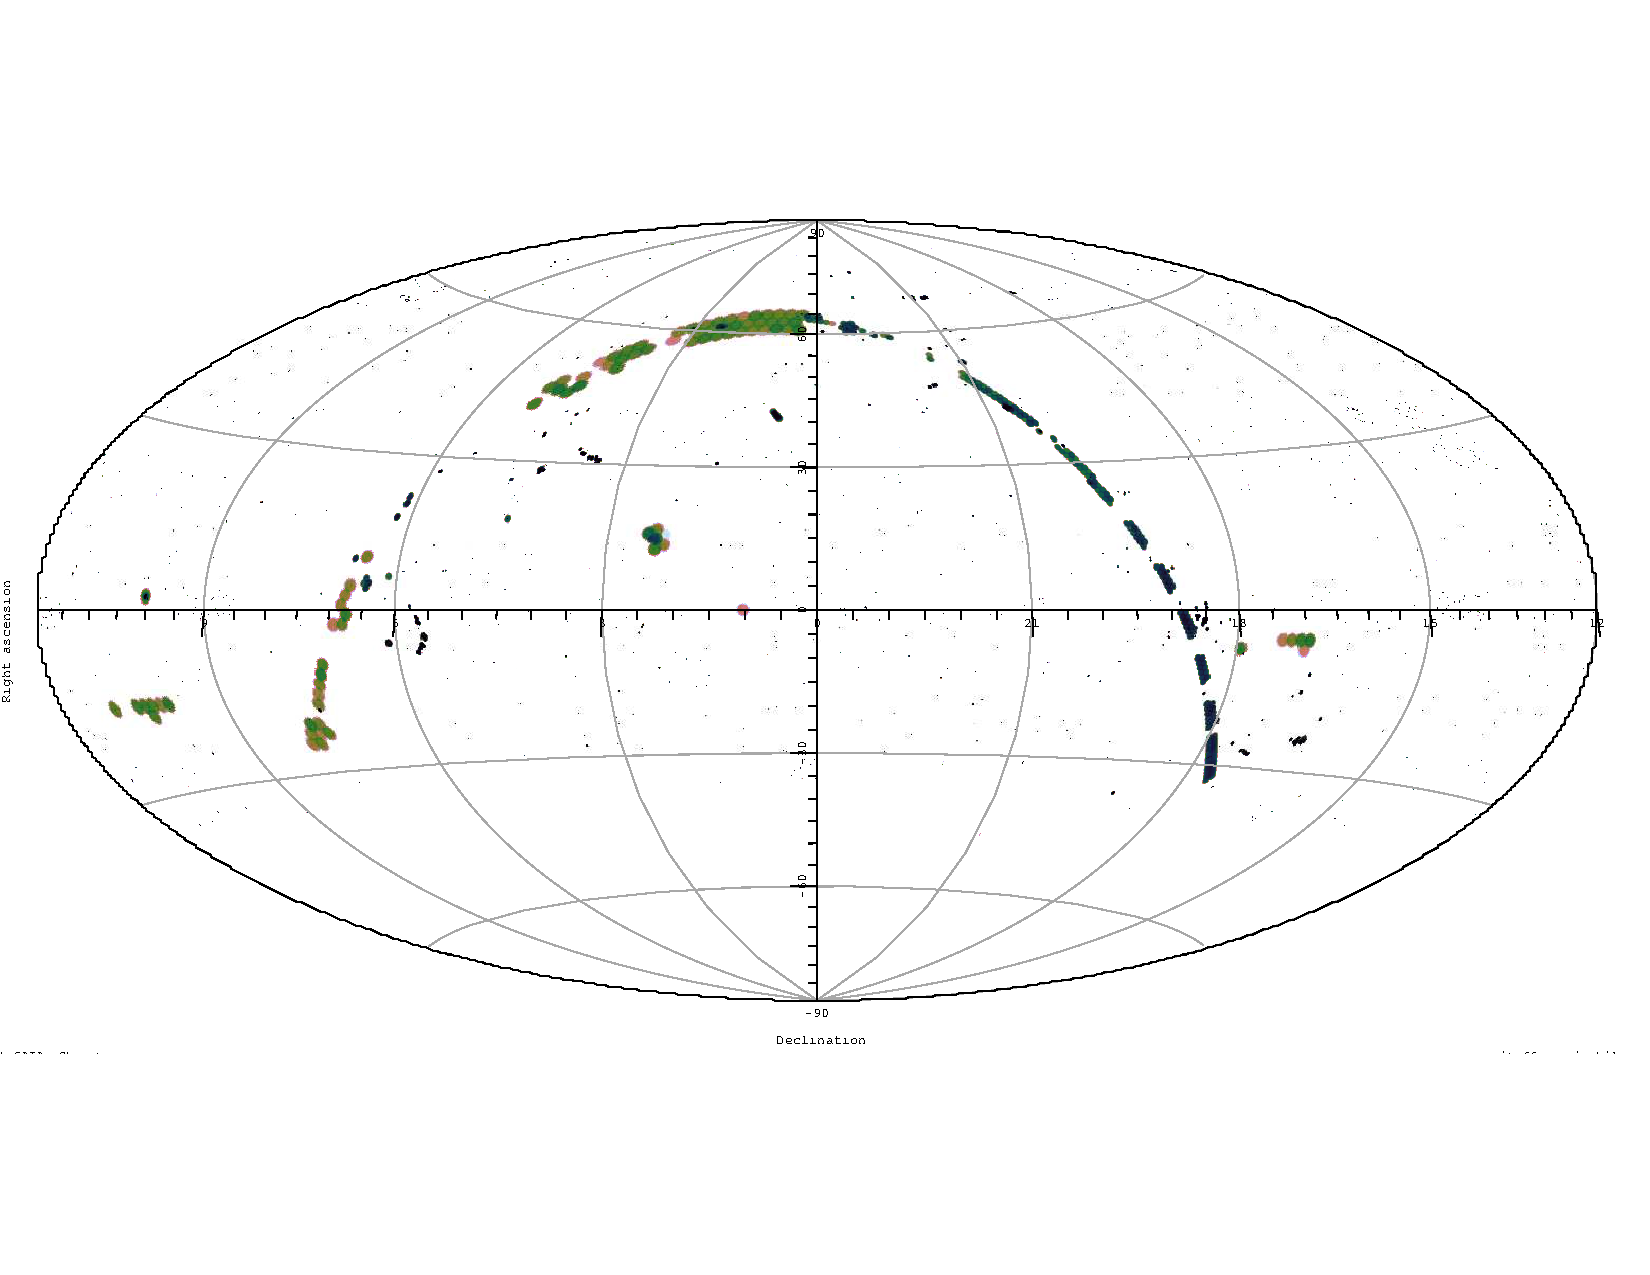
\includegraphics[width=0.9\linewidth]{legacy850-noise-aitoff}
  \caption{All sky noise map for this SCUBA-2 850\,\um{} legacy
    release. The large circular regions are 1 and 2 degree pongs,
    predominately observed near the plane of the galaxy. Small points
    are daisy observations towards sources scattered across the
    sky.}
  \label{fig:noise-aitoff}
\end{figure*}

\subsubsection{Included Observations}
This release includes publicly-released 850\,\um\ science
observations observed between 2011 February 2 and 2015 March
1. Observations from earlier than this were not included, as these
were taken in \emph{shared risk} mode while instrument commissioning
was still being conducted, and the data from that era are more
problematic \citep{SC19,Dempsey2010}.  Observations by the JCMT
Cosmology Legacy Survey \citep{Geach2013} are not included as they were
still proprietary until 2016 March 1. Observations by other SCUBA-2
JCMT Legacy Surveys
\citep[e.g.,][]{ChrysostomouJLS,GBS,SASSy,SONS,JPS}, as well as PI
projects, were included if they fell in the given time
range.

\note{Has any NGLS SCUBA-2 data been published (NO)? Need need proper
  SASSy refs. (There are none better as far as we know...)}

Pointing observations, and science observations from within the
appropriate time period that were judged to be of a low or
potentially-low quality, \emph{were} still reduced using this
standardised configuration\footnote{and are available for interested
  parties to download from the JSA}, but have not been included in the
co-added products (see \sref{sec:QA} for more detail on this).

In total, 21456 observations were reduced, of which 5161 are
\emph{science} observations, and 5521 were \emph{pointing}
observations (which were reduced but not co-added).  Of these
\emph{science} observations, 49 observations were marked as
\status{BAD} and excluded from the co-additions by our manual QA
process.\footnote{A further 390 were marked as
  \status{QUESTIONABLE}. This population were then examined further,
  and it was felt that these were all of high enough quality to
  include.}

\subsubsection{Coadds and catalogs}
These 5161 \emph{science} observations were successfully reduced onto
2930 distinct tiles, and 5519 \emph{pointing} observations were
reduced individually onto 263 distinct HEALPix tiles.

After excluding observations marked with a QA state of \status{BAD},
co-addition of the remaining 5059 science observations produced 2849
co-added tiles. The observed area within these tiles covers a total of
0.24 steradians (789.78 square degrees, or 1.9 per cent of the total
sky).

The individual observations and the co-added tiles are both available
to download from the JCMT Science Archive at CADC.

Source detection was carried out on all of the co-added tiles, and this
detected emission in 2.91E-4 steradians (0.96 square degrees, or 0.12
per cent of the observed area) of the co-adds.


\begin{deluxetable*}{lrrrrrr}
\tablecaption{Types of observation included in this
  release.\label{tab:typesobs}}
\tablehead{\colhead{Type} & \colhead{Number obs.} & \colhead{Total obs. time} & \colhead{Distinct tiles} & \colhead{Number coadded obs} & \colhead{Total coadd time} & \colhead{Distinct coadd tiles}\\ \colhead{ } & \colhead{ } & \colhead{$\mathrm{h}$} & \colhead{ } & \colhead{ } & \colhead{$\mathrm{h}$} & \colhead{ }}
\startdata
All & 21456 & 6414.4 & 4403 & 10256 & 5691.6 & 4143 \\
Science & 12586 & 5908.9 & 4185 & 10256 & 5691.6 & 4143 \\
Pointing & 8870 & 505.5 & 292 & 0 & 0.0 & 0 \\
Cals & 2234 & 138.1 & 22 & 60 & 4.8 & 14 \\
JLS & 6135 & 3636.7 & 2156 & 6015 & 3569.8 & 2145 \\
EC30 & 56 & 6.6 & 16 & 56 & 6.6 & 16 \\
PI & 4217 & 2134.2 & 2329 & 4181 & 2117.0 & 2303
\enddata

\end{deluxetable*}



\subsubsection{Noise statistics}
\todo{Recalculate with final released maps, and check for errors}

Because the observations used here are from a wide variety of projects
aiming for a variety of noise levels, our noise maps are extremely
heterogenous. Figure~\ref{fig:noise-aitoff} shows the all-sky
distribution of our noise maps. Table~\ref{tab:noises} shows the area
of our co-adds which has a noise level below various common
values. This is calculated by summing the number of
pixels which have a noise value less than or equal to a given limit.


\begin{table}
\centering
\begin{tabular}{l c r l}
  \hline
  mJy/arcsec$^{2}$& mJy/beam  & \multicolumn{2}{c}{Area}\\
                &          &  Sq. Deg. & Percent. \\
  \hline
  1  & 229.5& 740.7 & 94\% \\
  0.5  & 114.7& 585.4 & 74\% \\
  0.25  & 57.4& 246.0 & 31\%\\
  0.1 & 22.9& 71.8 & 9.0\%\\
  0.05 & 11.5& 37.0 & 4.7\%\\
%  0.01 &2.3 & 0.5 & $<$0.1\%\\
  \hline
\end{tabular}
\caption{Areas of the release which have an RMS noise less than or
  equal to the given value. \label{tab:noises} }
\end{table}

\section{Example regions}
\subsection{G34.3}
\begin{figure*}
  \centering
  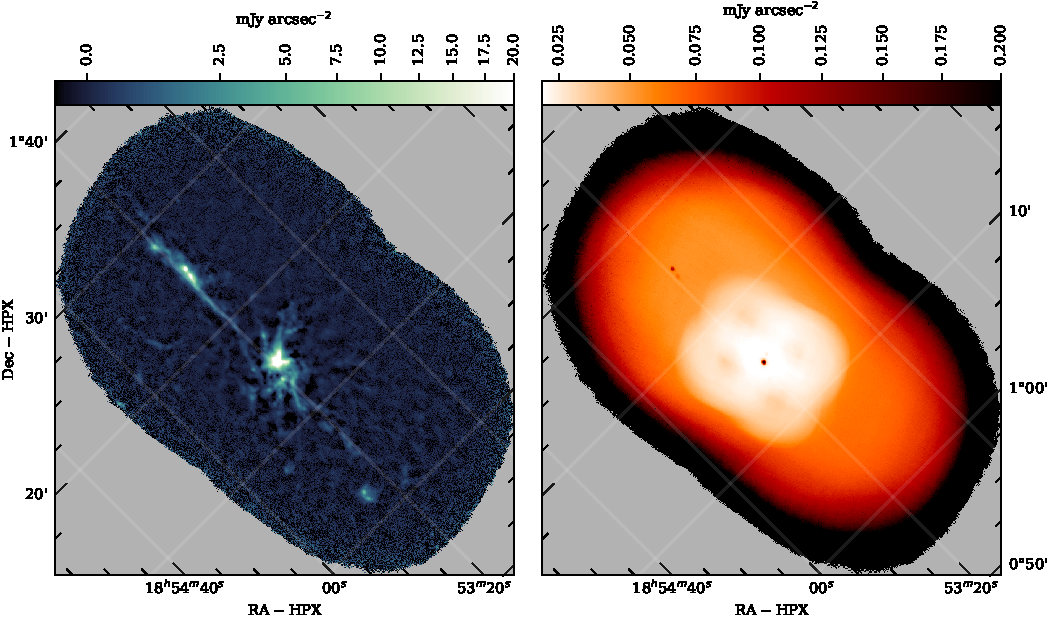
\includegraphics{tile30318-g34-coadd-noise.pdf}
  \\[3mm]
  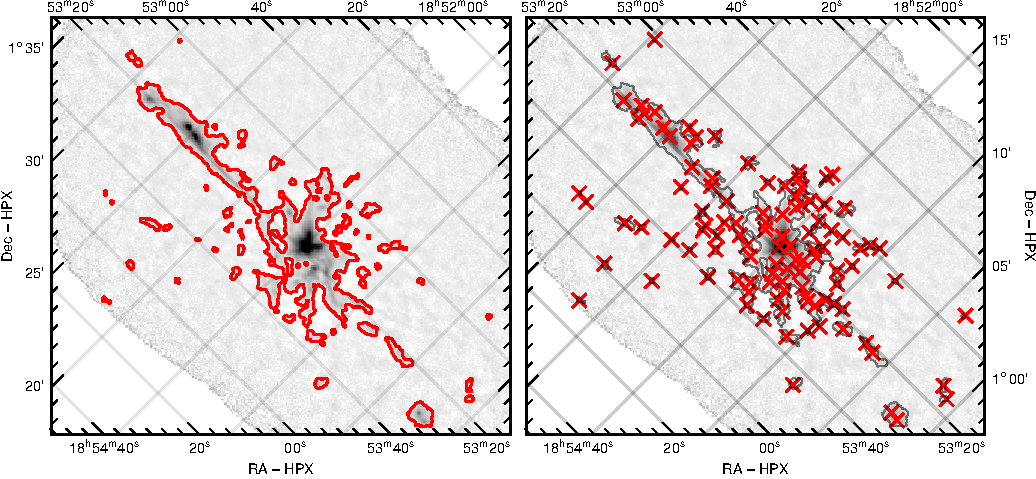
\includegraphics{tile30318-g34-extent-peak.pdf}
  \caption{Examples of the coadd, noise map, extent catalogue and peak
    catalogue towards tile 30318 containing the high mass star forming
    source G034.27+0.15}
  \label{fig:g34-3}
\end{figure*}
\subsection{CRL\,618}


\section{HEALPix grid}

To produce a uniform reduction of all public data, it is necessary to
have a suitable scheme for dividing the sky into pre-determined tiles
and pixels to grid the data onto.  The scheme needed to be well
defined in advance, without reference to the position of existing
observations, for consistency and in order to be able to easily
incorporate further data as they become public.  The tiling scheme
which was chosen is that offered by HEALPix \citep[Hierarchical Equal
Area isoLatitude Pixelization,][]{Gorski2005}, commonly used in
cosmological fields.  The HEALPix system starts by dividing the sky
into 12 facets, and then recursively divides these cells in four at
each higher resolution level.  There are two standard numbering
schemes used with HEALPix, of which the ``nested'' scheme has been
used to label tiles in this release, for convenience with the HPX
projection and compatibility with Virtual Observatory systems such as
MOC \citep[Multi-Order Coverage,][]{2013ASPC..475..135F}.

Pixels within the individual tiles also use the HEALPix grid, which
ensures that the pixelization is continous between each tile and the
adjacent tiles.  This has the advantage that the tiles can be joined
simply by abutting them.  This is done via the HPX projection
\citep{Calabretta2007} which allows the the HEALPix grid to be used
for conventional 2D FITS images.

While HEALPix has the advantage that all pixels have the same area,
the trade off is that the pixels are not all square: they can vary in
width and height while maintaining the constant area.  There are also
discontinuities in the angle of the grid lines at some facet
boundaries.  This is largely a display problem, as although image
viewers with a modern WCS implementation can handle files in the HPX
projection, the grid lines, and therefore astronomical sources also,
will appear bent at these positions.\footnote{If you are concerned by
  the visual appearance of HEALPix maps in your display and wish to
  reassure yourself that any apparent distortion is only due to
  display issues in your image viewer, we would recommend verifying
  the shape and position by contouring the map over a tangent plane
  map.}


\begin{table}
  \centering
  \begin{tabular}{ r l}
    \multicolumn{2}{c}{HEALPix parameters}\\
    \hline
    Tile size & $\sim$ 1\degr square \\
    Tile $N_\mathrm{side}$ & 64 \\
    Pixels in a tile  & 1024 $\times$ 1024\\
    Pixel area &  3.22$^{2}$ square arcseconds\\
    Pixel $N_\mathrm{side}$ & $2^{16}$ \\
    \hline
  \end{tabular}
  \caption{HEALPix parameters used for this release.}
  \label{tab:hpxpar}
\end{table}


\footnote{To re-grid one or more HEALPix tiles onto a standard RA-Dec
  projection, the Starlink \textsc{smurf} command \texttt{jsajoin} can
  be used \citep[][\ascl{1310.007}]{SUN258}.}

\section{SCUBA-2 data reduction}
SCUBA-2 observations are reduced using the Starlink SMURF programme
\texttt{makemap}. In brief, this is an iterative process that divides
the dataset into various instrumental and astronomical signals. There
are an extremely large number of user-adjustable parameters that can
affect the final map, depending on the science goals of the users and
the structure of the astronomical emission observed. \note{For example, a
cosmologist interested in detecting only faint point sources in a
primarily blank map would use a distinctly different set of parameters
from a galactic astronomer looking at bright, extended and
structurally complex emission.} For full details on the SCUBA-2 map
maker, please see \citet{Chapin2013}.


%Redraft this paragraph -- more paper-esque.
To guide astronomical users, the JCMT-supported Starlink software
comes with a series of standard configuration files for a variety of
common science cases.
% Although all JCMT observations are run through an automated pipeline
% every night \citep{2011scuba2dr,2015oracdr}, these reductions rely
% on the PI of the project selecting an appropriate reduction `recipe'
% for their science goals.
These standard configuration files can produce very poor results when
used on an inappropriate observation -- for example, the standard
SCUBA-2 configuration file used for calibrator observations is tuned
to expect a bright, compact source at the centre of the map. If used
by mistake on a blank field this recipe could easily create \emph{fake
  emission} in the form of large bloom-like structures. Avoiding this
sort of error was the paramount consideration when selecting the
configuration parameters.

Given the nature of SCUBA-2 data reduction algorithms, the main focus
in developing this \emph{legacy} configuration was on maximising the
confidence that could be placed in detection of emission, at the
expense of not attempting to recover large scale structures.

These observations were reduced using Starlink, Starjava and ORAC-DR
software developed between versions 2014A and 2015A. Interested
parties seeking to replicate these results can do so by checking out
the version of the code tagged as `2015A-legacy' release in the
Starlink code repositories\footnote{(See
  https://github.com/Starlink/starlink,
  https://github.com/Starlink/starjava and
  https://github.com/Starlink/ORAC-DR).}.


\subsection{Details of our chosen configuration file}

\note{Harriet suggests we might want an additional appendix, and the
  following sentence in this paragraph ``An expanded explanation of
  the SCUBA-2 mapmaker and its advances since Chapin et al. 2013 can
  be found in appendix B." with additional information in an
  appendix'').}



For the exact configuration file used in the legacy reduction see
appendix A. In this particular reduction, after the initial
pre-processing stage, the SCUBA-2 mapmaker recipe performs 5
iterations in which the astronomical signal is retained rather than
being removed (as in a normal iteration) prior to starting the next
iteration (specified using \texttt{ast.skip=5}). These initial
iterations allow the reduction process to focus on creating a mask
that identifies any unusually bright region. This is useful since such
regions may cause ringing in subsequent estimates of the low frequency
noise in each bolometer. During these iterations ``bright'' pixels are
taken to be those with a signal to noise ratio greater than 5.0, plus
any other pixels that are attached contiguously to such pixels down
the an SNR of 3 (specified by using \texttt{flt.zero\_snr=5} and
\texttt{flt.zero\_snrlo=3}).

During all iterations an atmospheric correction is applied and data
are filtered to remove any features on scales larger than 200". In
addition to this a separate common mode model is produced for each
subarray (specified with \texttt{com.perarray=1}). Having a separate
common mode estimate per sub array prevents artificial flux (also
known as ``fake blooms'') being introduced into the map where the
common modes vary significantly and are not well represented by a
single common mode. The disadvantage with having a separate common
mode for each subarray is that the reduction is limited to recovering
emission structures that are on the same scale or less than the
subarray size (approximately 200").

After the initial five iterations the recipe then performs up to 20
further iterations with all the models (specified by
\texttt{numiter=-25}; the initial 5 iterations plus these additional 20
iterations containing all models). Each of these remaining iterations
removes the astronomical signal from the residuals prior to starting
the next iteration. However, to prevent instabilities in the iterative
process, this subtraction only occurs within regions corresponding to
bright sources.  The mask identifying such sources is creating in the
same way as the mask used by the low frequency noise filter (``FLT''
model): source pixels are taken to be those with a signal to noise
ratio greater than 5.0 (plus any other pixels that are attached
contiguously to such pixels down the an SNR of 3 (specified by using
\texttt{ast.zero\_snr=5} and \texttt{ast.zero\_snrlo=3}).

The map maker exits before the 20th iteration if the \texttt{maptol}
parameter --- the change between maps --- has reached a mean value of 1\%
of the noise level (specified by \texttt{maptol=0.01}).


% See appendix \ref{app:config} for the full configuration file. Some of
% the most important details are described below:

% Our mapmaker configuration first of all performs 5 iterations without
% creating an astronomical model of the source. \note{Harriet\&DSB: do
%   we have a short explanation of do we do this again?}. It will then
% perform up to 20 further iterations with all the models, but will exit
% before that point if the 'maptol' parameter has reached a mean value
% of 0.01.

% In order to decrease the production of fake 'blooms' of emission in
% the final map, we produce a separate COMMON mode model for each
% subarray (\texttt{com.perarray=1}). While this produces more reliable
% output (appropriate for this project which has comparatively minimal
% by eye checking of data), it has the effect of removing structure
% scales that are larger than the subarray size.

% \note{zero snr and zero snrlo: need a proper explanation for these}
% We also set the 'AST' and 'FLT' zero\_snr and zero\_snrlo values.

Figure \ref{fig:crl618-example} shows a reduction of a single
observation towards a standard calibrator, reduced using both the
legacy configuration file presented here (in an HPX projection), and
with the standard calibration reduction configuration `bright compact'
on the tangent plane projection.

\begin{figure}
  \centering
  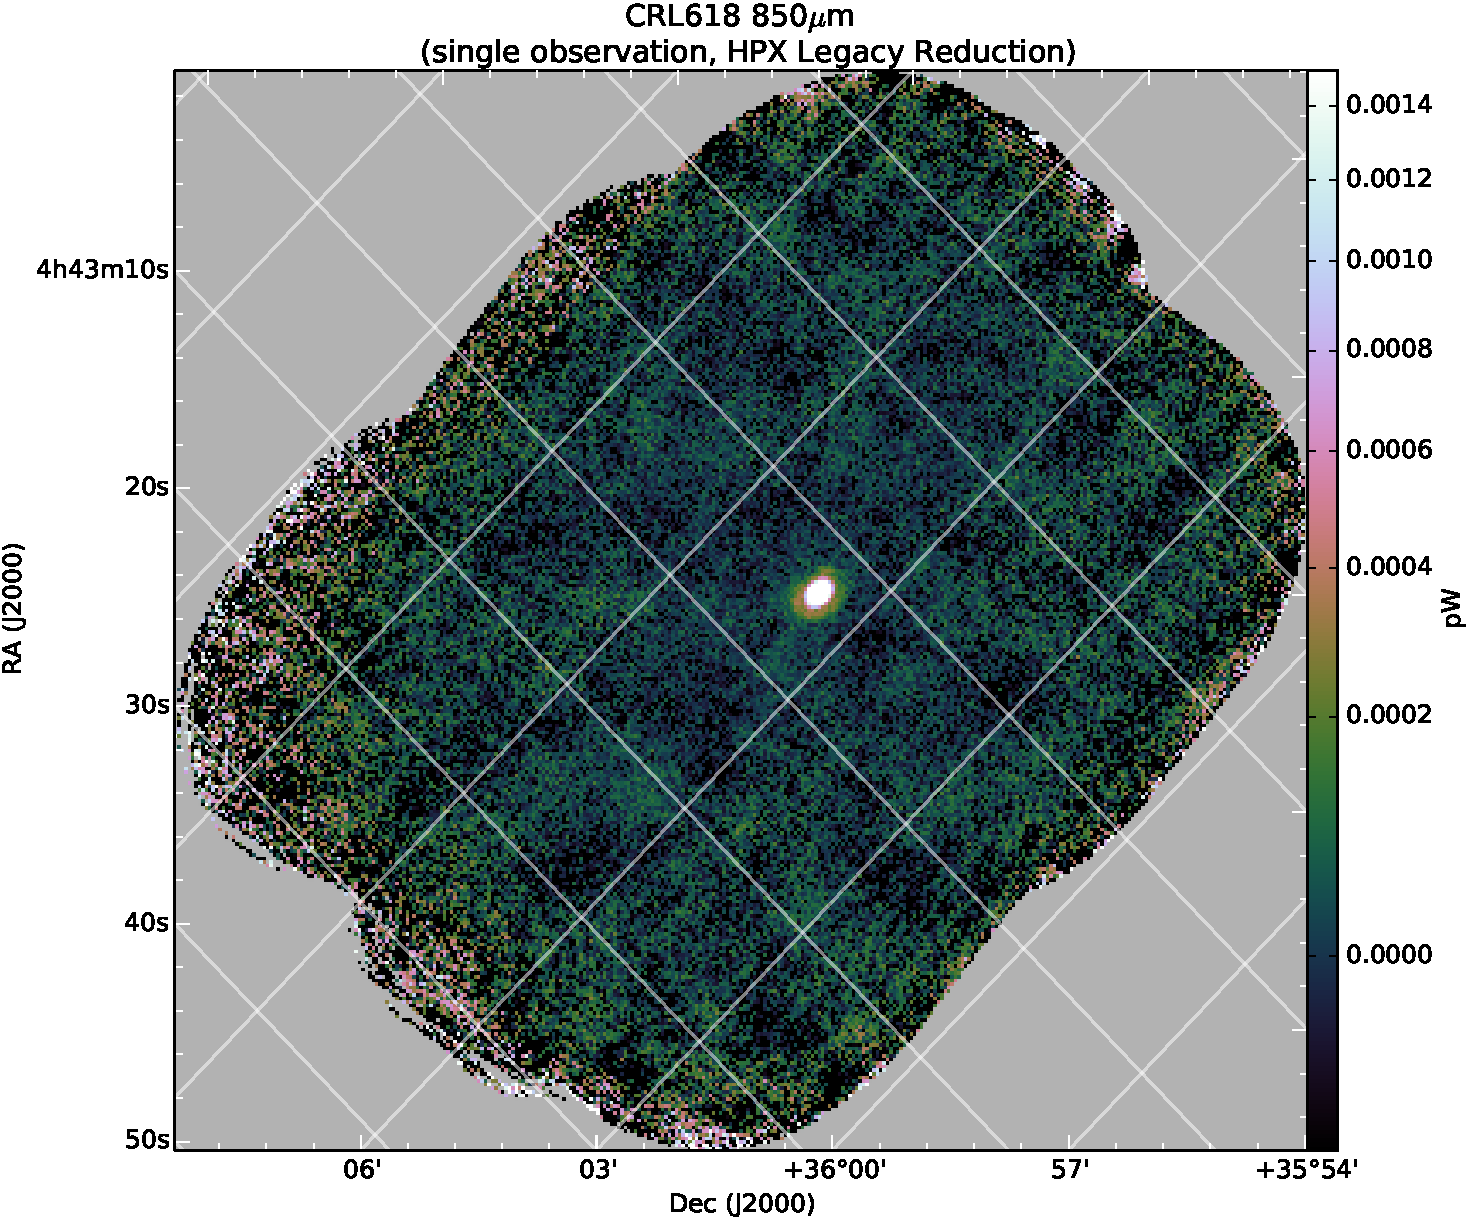
\includegraphics[width=0.45\linewidth]{crl618_example_legacyred}
  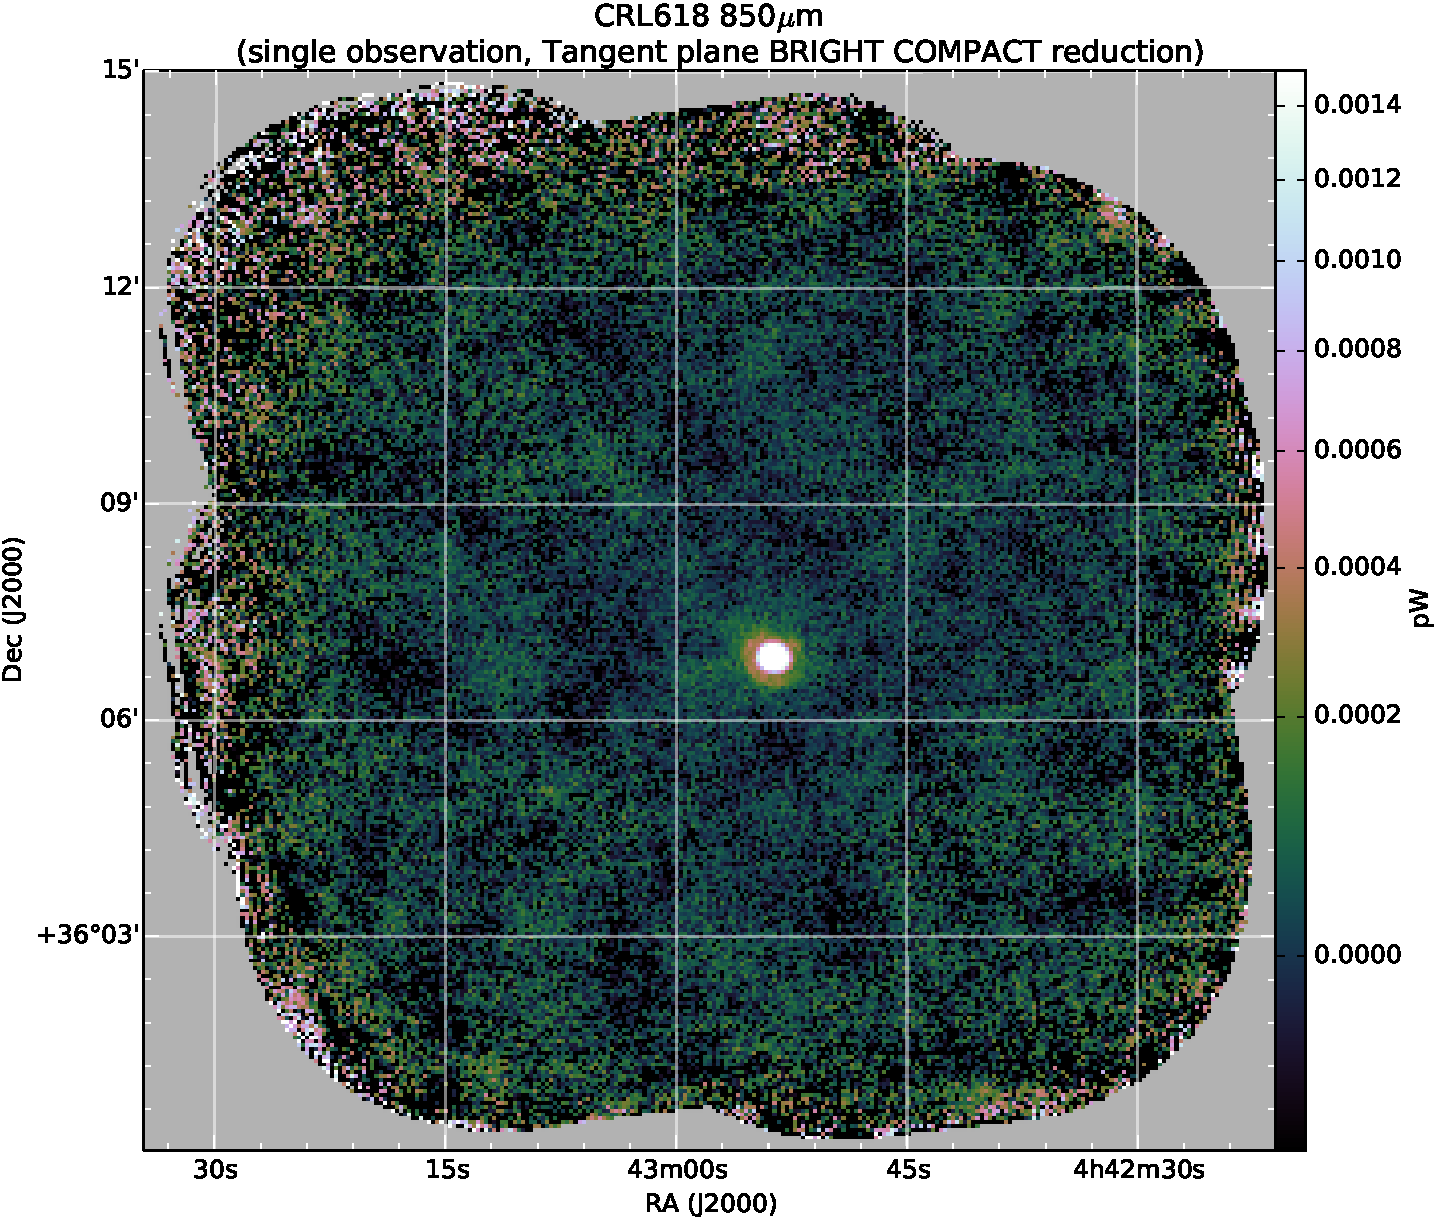
\includegraphics[width=0.45\linewidth]{crl618_example_bcred}
  \caption{Left: A legacy 850\,\um{} reduction of a single observation
    towards the JCMT standard calibration source CRL 618. Note that
    the pixel axes are at 45 degrees to the RA and Dec axes. As each
    pixel in the map is truly shaped like a diamond (i.e. a stretched
    square), the distortion introduced by an image viewer that
    displays every pixel as a square causes the source to appear
    ellipsoidal. Right: For comparison, a standard non-HEALPix tangent
    plane reduction with the Bright Compact configuration is shown for
    the same source. Here the source appears more circular. Both maps
    are shown in uncalibrated units of pW on the same scale. These
    maps cover two tiles.}
  \label{fig:crl618-example}
\end{figure}


Figure \ref{fig:omc1-example} shows a reduction of a single
observation towards the complex, bright and extended OMC-1
region. \todo{ Should this have a comparison with e.g. a GBS
  reduction of this region, to show the difference in size scales?
Or leave that for later}.

\begin{figure}
  \centering
  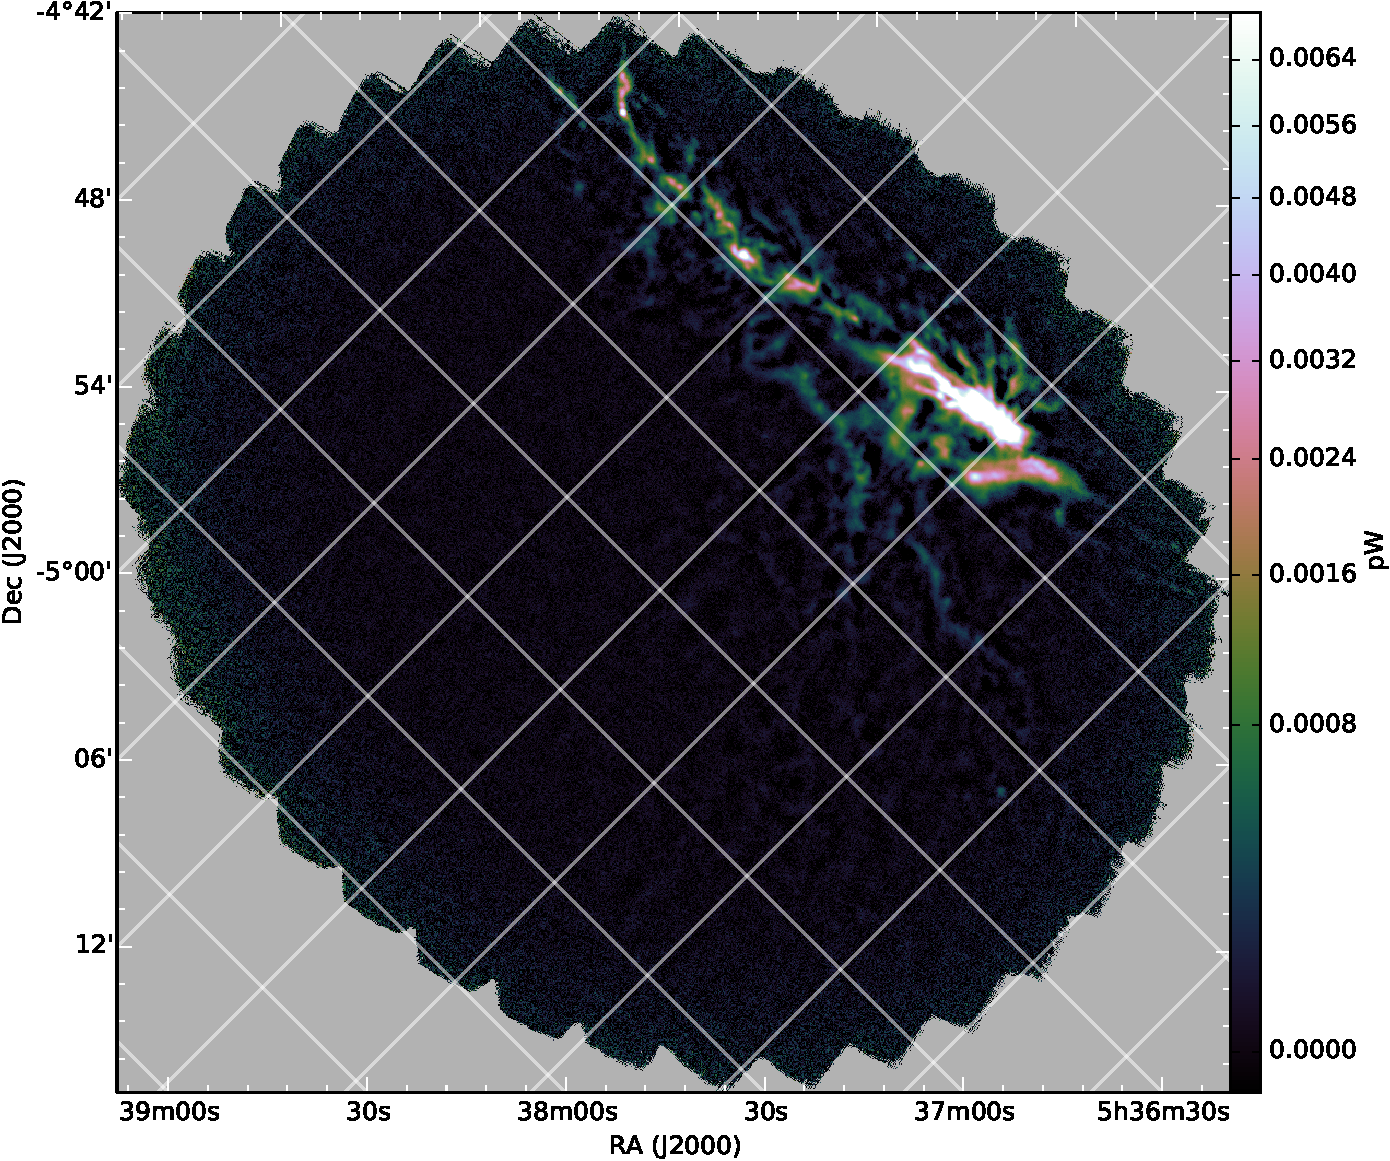
\includegraphics[width=0.6\linewidth]{omc1_example_legacy}
  \caption{A legacy 850\,\um{} reduction of a single
    observation(observation 93 from 2012-08-17) towards the OMC-1
    source. This observation overlapped with 3 tiles: 22805, 21439 and
    21438. }
  \label{fig:omc1-example}
    \end{figure}


\subsection{Co-adding of tiles}
All observations towards a given tile that passed QA were co-added,
using the \texttt{makemos} applications from Starlink's
\texttt{ccdpack} \citep[][\ascl{1403.021}]{SUN139}. This co-adding was
carried out as a variance-weighted mean. No despiking was
performed. The variance map for the co-added tile is also produced.

\todo{Picture of a coadded tile? Both data and noise. Pick something
with Daisy and pongs in it, as a comparison.}


%\todo{Each observation is gridded into pre-defined tiles. Are they
%  extinction corrected at that point? Unlike HARP processing
%  \citep{2015ACSISDR}, observations can be reduced independently and
%  then co-added. Extinction correction can be applied during co-adding
%  phase? How well are edge-effects handled by variance weighting?}


\section{QA}
\label{sec:QA}
\todo{SHORTEN}

\subsection{Standard JCMT QA States}
All observations taken by the JCMT are classified as \status{GOOD}
(the default), \status{BAD}, \status{QUESTIONABLE}, \status{JUNK} or
\status{REJECTED}. We included \status{GOOD}, \status{QUESTIONABLE}
and \status{REJECTED} data in our co-adds. The \status{REJECTED} state
is used by the JLS teams to indicate that a particular observation did
not meet their particular QA criterion but the data are otherwise
usable. The \status{QUESTIONABLE} state was originally designed to be
a transient state that would be resolved into either \status{BAD} or
\status{GOOD} after analysis, but in practical terms there was not a
workflow to ensure this, so some observations have this flag in the
archive.

Usually (in the standard nightly reduction pipelines)
\status{QUESTIONABLE} data is treated as if it is \status{BAD} for the
purposes of co-adds. However, due to our second QA stage for this
release, we chose to include it as long as it passed our special
legacy QA.

\subsection{Legacy Release QA}
%Description of process. Examples of observations we threw out.

\todo{In this what?}
Every reduced file included in this has been marked as \status{GOOD}
by a member of the JAC team. This quick `by-eye' assessment was simply
done on a image of the reduced map. This QA process was designed to
avoid: a) `blooms' or `blobs' of fake emission that can sometimes be
produced at the edges of the map by the mapmaker.  b) identify the
most problematic observations that had missed being flagged under the
telescope standard QA process.

This sort of process is of course subjective, and some of the
observations that we excluded might be usable on further
examination. However, as with all of this process, the focus for this
release has been to ensure a high quality, even at the expense
of completeness. All of the HEALPix-gridded legacy-reduced
observations are available to the community in the JSA, regardless of
our QA analysis of them, so interested users can evaluate the full
available data themselves.

%
\subsection{Examples of BAD observations}
- explains why we did it.


\section{Calibration}



\begin{itemize}
\item show images the standard calibrators.
\item comparison with `standard' calibrator reductions
\item effect of pixel size on fluxes. Per, Jess \& Daniel may have
  something. Doug J. and GBS did an analysis on this as well.
\item effect of pointing errors on fluxes.
\item Our uncertainty in the final flux.

\item PICTURES: calibrators, comparison with bright compact and 1
  arcsec. Examples of the coadded deep maps of all of our
  calibrators?.
\end{itemize}

The calibration of these data follows the approach used in the
standard SCUBA-2 calibration paper \citep{Dempsey2013}. In brief, a
Flux Conversion Factor (FCF) is derived from observations of standard
calibrators of known brightnesses, which is then used to convert from
the instrumental units of pW into astronomical units. For the
JCMT-LR1, an average FCF was derived for the standard calibration
observations taken in our time period and reduced with the legacy
configuration described above.  The reductions of each observation
were left in the instrumental pW units, and the FCF correction was
applied to the co-added tiles to produce units of
mJy\,arcsec$^{-2}$. For more information about FCFs and their
derivation, please see \citet{Dempsey2013}.

Three commonly used SCUBA-2 calibrators have been analysed to derive
an appropriate arcsecond FCF for this dataset. These are Uranus,
CRL\,618 and CRL\,2688. Note that the Uranus calibration observations
are not part of the standard legacy release themselves, as
observations of moving targets were not included in this release.

An arcsecond FCF was derived for the JCMT-LR1 850\,\micron\ reduction
of each calibration observation towards these three
sources.\footnote{Observations that had been marked as poor quality
  during QA were not included in the following analysis.}  The Uranus
observations from the time period covered by this release had been
separately reduced using the same SCUBA-2 configuration and pixel
size, but not onto a HEALPix grid due to being a moving target. The
PICARD (\citealp{SUN265}, part of ORAC-DR, \citealp[][\ascl{1310.001}]{SUN230})
recipe SCUBA2\_CHECK\_CAL\footnote{see
  \url{http://www.starlink.ac.uk/cgi-bin/htxserver/sun265.htx/sun265.html?xref_SCUBA2_CHECK_CAL}}
was used to derive this arcsecond FCF.

The mean and standard deviation of the derived FCFs were calculated,
using a 5-sigma clipped mean to remove extreme outliers. This removed
observations with an FCF higher than 3.24 and lower than 1.72 (see
Fig.~\ref{fig:calibhist}). The final average value is:

\begin{equation}
\mathrm{FCF}_{\mathrm{arcsec},850} = 2.48 \pm 0.15\ \mathrm{Jy}\ \mathrm{pW}^{-1}\  \mathrm{arcsec}^{-2}.
\end{equation}

\begin{figure}
  \centering
  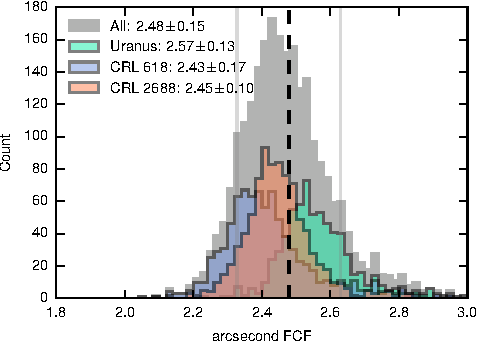
\includegraphics{lrvalues-histo}
  \caption{Histogram of FCFs, both for all sources (light gray) and
    separately for each source. The derived average FCF is shown as
    the dashed vertical line, with the $\pm$1s.d. shown as the light
    gray lines to either side.}
  \label{fig:calibhist}
\end{figure}

The co-adds in this release were calibrated using this mean FCF.  This
standard deviation represents a 1-$\sigma$ uncertainty of
approximately 6 percent. All co-adds were calibrated using the same
FCF. If it is wished to undo the calibration and redo with a different
value, please simply divide the dataset by this FCF, and then
recalibrate using the FCF of your choice. Similarly, this can be done
with any flux values quoted in the catalogues derived from the
co-adds. A PICARD recipe (SCUBA2\_UNCALIBRATE\_DATA\footnote{see
  \url{http://www.starlink.ac.uk/cgi-bin/htxserver/sun265.htx/sun265.html?xref_SCUBA2_UNCALIBRATE_DATA}})
is also provided as a convenience -- this will set the appropriate
units within the dataset.

For comparison, the usual `canonical' 850\,\micron\ arcsecond FCF used
in the JCMT's nightly reductions is $2.34 \pm 0.08 \mathrm{Jy}\
\mathrm{pW}^{-1}\ \mathrm{arcsec}^{-2}$ \citep{Dempsey2013}. This is
approximately 6 percent lower than the value used here, and was
derived using the `bright compact' SCUBA-2 configuration on 1
arcsecond pixels (in comparison with the 3.22$\times$3.22 arcsecond
pixels in this release), on with observations taken from 2011 to
XX. Fig.\,\ref{fig:lr-caldb-histo} shows the comparison between the
histograms of bright compact derived FCFs and the legacy release
derived histogram, for the same
observations. Fig.\,\ref{fig:lr-caldb-scatter} shows the scatter plot
of each bright compact FCF vs the legacy release FCF for each
observation. Broadly speaking, we see a linear relationship between
the two derivations of FCF.
\begin{figure*}
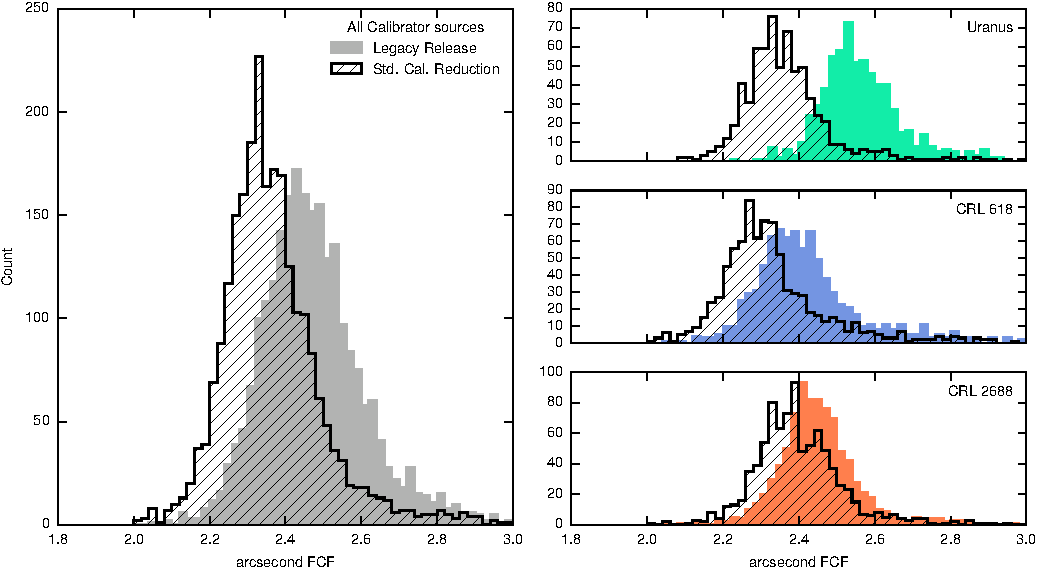
\includegraphics{legacyFCF-caldbFCF-histograms.pdf}
\caption{\todo{Probably remove?}Comparison between the histograms of
  arcsecond FCFs derived from the legacy reduction and the standard
  JCMT SCUBA-2 calibrator reduction, for the same observations.
  These are shown both overall and broken down by source (CRL 618,
  CRL 2688 and Uranus). Note that the LR Uranus maps were \emph{not}
  reduced onto a Healpix grid, but did use the same pixel area and
  \texttt{makemap} dimmconfig as the other LR reductions.\label{fig:lr-caldb-histo}}
\end{figure*}
\begin{figure}
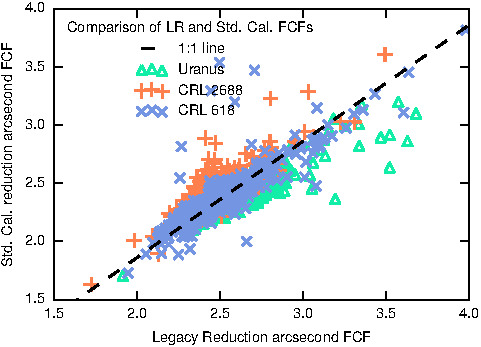
\includegraphics{legacyFCF-caldbFCF-scatter.pdf}
\caption{Comparison between the FCFs derived from the legacy release
  reductions, and those derived from the standard JCMT SCUBA-2
  calibrator reduction. The dashed line indicates a one-to-one
  relationship, offset by the difference in the derived FCF used for
  calibrating the legacy release (2.48) and the canonical FCF from
  \citet[2.34]{Dempsey2013}. \label{fig:lr-caldb-scatter} }
\end{figure}


To show the variation seen in the individual FCFs, we provide for
reference plots of the histogram of the FCFs
(Fig.~\ref{fig:calibhist}), the variation in FCF with opacity
(Fig.~\ref{fig:calibvstrans}) and the variation in FCF with date
(Fig.~\ref{fig:calibvstime}). No correction to the FCF for sky opacity or date
was made in this release.

\begin{figure*}
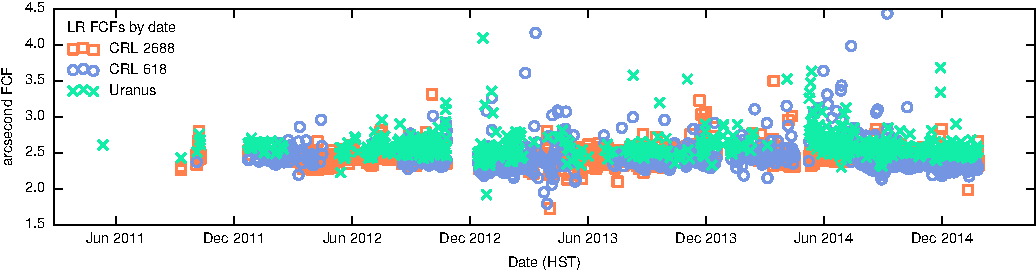
\includegraphics{legacyFCF-vs-date.pdf}
\caption{The arcsecond FCFs derived for the legacy reductions of CRL
  618, CRL 2688 and Uranus, shown against time. Although there is a
  large scatter and some hints of variation , it can be seen that there is not
  clear overall dependency with time.\label{fig:calibvstime}}
\end{figure*}
\begin{figure}
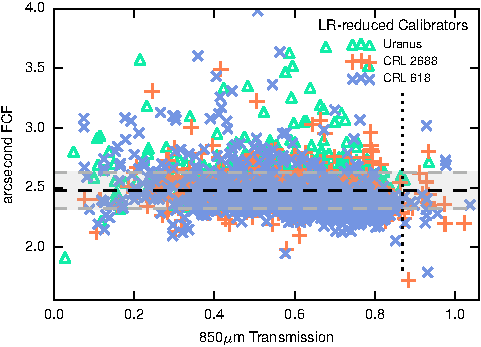
\includegraphics{legacyFCF-vs-transmission.pdf}
\caption{The legacy arcsecond FCFs derived from CRL 618, CRL 2688 and
  Uranus, shown against the 850\micron\ atmospheric transmission
  during the observation. Horizontal lines indicate the derived mean
  and standard deviation of the FCFs. A vertical line indicates the
  cut off in transmission applied to the coadds in this data
  set. \label{fig:calibvstrans}}
\end{figure}


\subsection{Uncertainty}

The standard deviation of the sample of derived FCFs represents the
minimum uncertainty in this calibration. In addition, we should take
into account the standard error in the sub-mm flux of
Uranus. \citet{Dempsey2013} quote this as $\pm$ 5 percent. Taken
together in quadrature, this gives an overall estimated error of
$\pm$8 percent.



\section{Noise}

\begin{itemize}
\item Noise maps: overlaps work fine, show an example? 
\item Copy COHRS pixel distribution graph?
\item noise on each pixel, noise vs integration time.
\item High noise towards bright sources.
\end{itemize}

\subsection{Histogram of noise in all pixels}
\begin{figure}
  \centering
  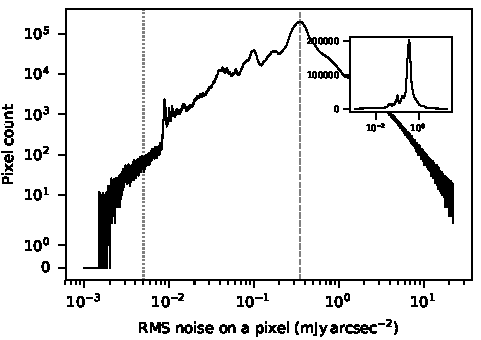
\includegraphics{coadds-noise-histogram.pdf}
  \caption{Histogram of the RMS noise on each pixel in the coadds. The
    main plot is shown with a log y-axis scale, and a linear y-axis
    scale is shown in the inset. Note that no trimming of observations
    is done for this, so the noisy edges of the SCUBA-2 observing
    patterns are included. The noise is taken from the makemap
    produced variance array, which uses the scatter of input data
    points to estimate the variance of a given pixel while reducing
    the raw time series onto a sky map.}
  \label{fig:histonoise}
\end{figure}
\subsection{Noise vs integration time}
% this is harder to do -- how to do a scatter plot of with billions of
% points.. 2-d histogram instead? produce in same way as the noise
% coadds.
\subsection{Anomalous variance array values towards bright sources}
% USe OMC-1 and cRL 618 as examples? Also visible in G34.3 shown earlier.

\section{Pointing}
\begin{figure}
  \centering
  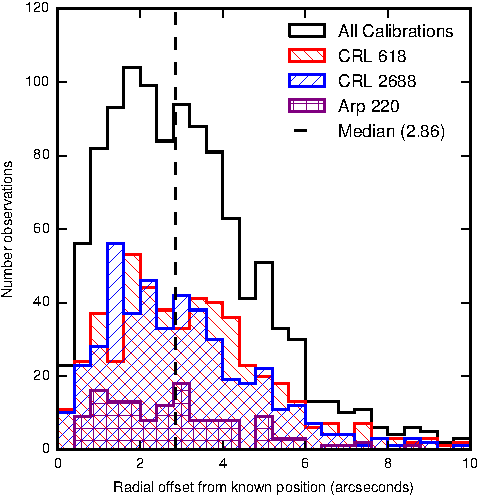
\includegraphics{pointing-offsets-by-source.pdf}
  \caption{Histogram of the total magnitude of the position offsets
    found in the JCMT Calibrator sources, with the 3 most common
    sources shown separately. The median value of 2.86\arcsec{} is
    indicated on the plot. Note that a small number of observations
    with anomalously high values are not shown in the plot, although
    they were not cropped before calculating the median.}
  \label{fig:pointing}
\end{figure}

The JCMT usually quotes a pointing offset of apporixmately 2\arcsec{}
in x and y, corresponding to an average radial offset of
2.9'\arcsec{}, which is confirmed within this dataset.
The pointing of this falls within the JCMT expected average 2\arcsec{} offset
from the source. \todo{Get citation for JCMT expected average pointing
  issue. Probably website or Jenness 2011}

\note{CRL 2688 needs re-reducing due to the issue in position.}
%\end{itemize}

\section{Catalogues}
The JCMT Legacy release includes emission catalogues generated from
each of the co-added maps. As we have an extremely diverse set of
astronomical regions (including blank fields, point sources and large,
complex extended structures), we did not feel it would be possible to
perform astronomical source finding and classification. Instead, this
release focused on identifying first of all \emph{regions of
  contiguous emission}, discussed here as \emph{extents}, and secondly
on \emph{identifying local maxima within those regions}, described
here as \emph{peaks}. The primary goal of these catalogues is to
ensure it is easy for astronomers to identify regions with secure
detections of emission.

We have chosen to use the Fellwalker algorithm \citep{Berry2015}, as
implemented in the Starlink CUPID \citep{cupid} package for this
analysis. Unlike the more commonly used ClumpFind which simply lays
discrete contour levels on the map and uses those to identify regions,
Fellwalker follows lines of ascent within the map to identify all
peaks of emission. We have found it to be robust and
easy-to-understand, and to produce intelligible results.

\subsection{Extents}

We have identified the regions of contiguous extended emission within
each tile by looking at the Signal-to-Noise maps of the co-added
tiles. We determined that we would consider all regions of contiguous
emission containing flux brighter than 5 sigma to be a single `extent'
for purposes of our reductions, if the region is larger in area than a
beam. We followed the source down to a noise level of 3 sigma.  Here,
a simple approximation of the beam was used (all sources larger than 9
pixels). We considered using a more complex approach, but noise spikes
in makemap maps do not appear to be found by this size. The main
source of false detections in our reductions would have been the
previously discussed problem of `false blooms of emission'
occasionally produced by makemap reductions, if we had not used a
by-eye approach for flagging the handful of problematic reductions and
removing them from the output.

The reduced observations, produced by SMURF's makemap routine, all
contain a variance array giving the noise towards each pixel, based on
the scatter of input data points to that pixel. Pixels with too small
a number of inputs to calculate a variance point are not included in
the individual maps. Our co-adding procedure uses this variance to
weight the input observations. We do see anomalously high noise
towards bright sources (see Fig.~\ref{fig:noise-bright-source} for an
example of this), however this is not at a level to prevent a signal
to noise 5 sigma detection.

\todo{Note on varying noise within tiles -- show some examples,
  explaining why its so necessary to use SNR instead of a
  representative noise when the noise varies across the tile.}

We used the Fellwalker algorithm as implemented in CUPID on an SNR map
to produce contiguous regions of emission and to identify the position
of the peak pixel within each map, and these outlines are available
both as a FITS format mask file, as a HEALPix Multi-Order-Coverage
file (MOC) and as a rough approximation by STC-S polygon. The
catalogue for each tile indicates the ID of the clump, the RA and Dec
of the peak pixel, the total flux contained within the entire extent,
the flux of the peak pixel, and the area of the entire extent. We also
include the approximation of the outline of the extent as an STC-S
polygon string. This can be plotted with software such as GAIA.



\todo{Example extent maps -- pick 3 showing a variety of different
  types of structure. Include a null detection?}

\subsection{Peaks}
In order to provide some information about the nature of emission
within the extents, this release includes identification of local
maxima within the extents. \emph{It is important to note that these
  should not in general be considered as point sources.} We identified
these points by running the Fellwalker algorithm (from Cupid) on the
extent map. The peak detections were not created from the SNR map, as
we could assume by only looking within the detected extents that we
were already looking at detected emission.

As our maps contain a varying noise, we used the mean noise across the
entire detected extent as a representative noise. We then used the
Fellwalker algorithm with that noise as the RMS value, and identified
as individual local maxima those which contained a peak of 5-$sigma$,
followed down to a noise level of 3-$sigma$, and with at least a
5-$sigma$ dip between them and neighbouring maxima. Our output
catalogue contains the ID of the peak, the RA and Dec of the peak
pixel, the flux in the peak pixel, and the ID of the extent the peak
was drawn from.

We decided not to include the outlines of all emission counted as
being within that object or clump, as we felt that would encourage
users to consider the peaks as being real, physical objects. Although
they may be in some cases, in many other cases the peak is simply a
local maxima within a complex molecular cloud. The `clump outlines'
produced by software such as CUPID always reflect the arbitrarily
chosen boundaries of dips and minimum heights, and should not be
assumed to represent physical objects without considerable further
modelling (\todo{SFG:Cite and further discuss the various papers
  highlighting the problems in clump numerology -- list is on
  laptop}.)


\section{Limitations of our reduction}


\subsection{Source Recovery: Comparison including fake sources?}
\todo{SFG: write this up properly}
\note{From LR1-releasenotes. Needs rewriting.}

Recent work by \citet{Mairs2015} indicates that
in SCUBA-2 reductions there is a significant difference between
recovery of sources inside and outside the AST mask. Sources that are
outside the AST-masked regions can have their flux considerably
underrepresented. The AST masked region can be thought of as roughly
the region containing detectable emission in the single observation,
based on the specific configuration parameters chosen. The effect is
dependent on the size of the source -- extended sources outside of the
masked regions are poorly recovered in this reduction. To identify the
regions masked in each individual observation, please look at the
QUALITY mask and see the following blog post on this:
\url{http://pipelinesandarchives.blogspot.com/2014/06/interpreting-scuba-2-map-quality-arrays.html}

Importance of detection inside vs outside the automask.

This issue does in fact affect all reductions, including those using
external masks defined from previous knowledge of the emission, but
is more problematic when automasking.

Detection of objects outside the masked region: point sources
recovered well, extended objects lose considerable flux.


\subsection{Size Scales}
We have excluded sizes scales larger than the sub array size from our
reduction. In addition, we have used a fairly aggressive large scale
filtering removing scales larger than 200 arcseconds.
\todo{Do we want some power spectra of this? not sure if they'd be very illuminating.}

\subsection{Negative Bowling}
Examples of the bowling in our maps.\todo{Harriet/David: good description of why this happens?}

% \section{Comparison with legacy surveys}

% \todo{A SCUBA-2 image from each survey alongside a Legacy Release
%   version. Which wavelengths? SASSy only has one published field
%   \citep{MacKenzie2011}. JPS and NGLS may not have any yet. GBS has a
%   few recent papers with \citet{Rumble2015} published for Serpens.}



\section{Conclusions}

\acknowledgments

The James Clerk Maxwell Telescope has historically been operated by
the Joint Astronomy Centre on behalf of the Science and Technology
Facilities Council of the United Kingdom, the National Research
Council of Canada and the Netherlands Organisation for Scientific
Research. This work was funded by the Science and Technology
Facilities Council.  Additional funds for the construction of SCUBA-2
were provided by the Canada Foundation for Innovation.

The work presented here was initially started by the Joint Astronomy
Centre, and latterly has been supported by East Asian Observatory.


\vspace{5mm}
\facility{JCMT(SCUBA-2)}

% Include software citations here again?
% Check if there is more.
\software{Starlink, SMURF, KAPPA, ORAC-DR}





\appendix


%% Probably more detailed than needed in a paper
\section{Mapmaker configuration}
\label{app:config}
The mapmaker configuration used for this release (known as a
\texttt{dimmconfig}) is shown here. Like most SCUBA-2 mapmaker
configuration files, it first sources the \emph{base}
\texttt{dimmconfig} file that sets up the basic values for a range of
options and then tweaks a subset of additional parameters or its
purposes. This file is shipped in the 2015A Starlink release. The
value of every configuration parameter used is written into the
history component of the file.

\begin{verbatim}
^$STARLINK_DIR/share/smurf/dimmconfig.lis

#  Less aggressive cleaning to cope with bright sources
noisecliphigh=10.0
dcthresh = 100

#  Don't want extended structure, so avoid problems with COM model by using
#  individual common-mode models for each subarray.
com.perarray = 1

#  Aggressive filtering.
flt.filt_edge_largescale=200

#  Allow bolometer noise to vary with time, and using a box filter to
#  determine mean noise in each box, in order to presevre as many samples
#  as possible.
noi.box_size=-15
noi.box_type=1

#  Use a maximum of 20 iterations
numiter=-25
maptol_mean=1
maptol=0.01

# new recommendations and using an ast model
ast.zero_snr = 5
ast.zero_snrlo = 3

ast.skip=5
flt.zero_snr=5
flt.zero_snrlo=3
\end{verbatim}

\section{Accessing the Legacy Release}
A brief summary of how to access the data, catalogues.


\bibliography{legacy-850um-paper}
\bibstyle{aasjournal.bst}


\end{document}
